\documentclass{beamer}
\usepackage[british]{babel}
\usepackage[utf8]{inputenc}
\usepackage{styles/jyumacros}
\usepackage[version=4]{mhchem}
\usepackage{textgreek}
\usepackage[absolute,overlay]{textpos}
\usefolder{styles}
\usetheme{jyu}

%change these to your own logos if needed (try and match sizes, otherwise, change sizes in Outer Theme file).
\titlegraphic{assets/coverlogo.pdf} %logo on the cover page
\newcommand{\smalllogo}{assets/small_white.pdf} %small logo on frames

%Personal info---------------------------------------------
\title{MARA-LEB}
\subtitle{An Insight into Nuclear Physics Experiments}
\date{20.8.2021}
\author[auth]{Jorge Romero}
\institute[inst]{University of Liverpool, Jyväskylän Yliopisto}
%----------------------------------------------------------

\begin{document}
\begin{frame}
\titlepage
\end{frame}

\begin{frame}{JYFL Acclab}
    \centering
    \vspace*{4em}
    \hspace*{-3em}
    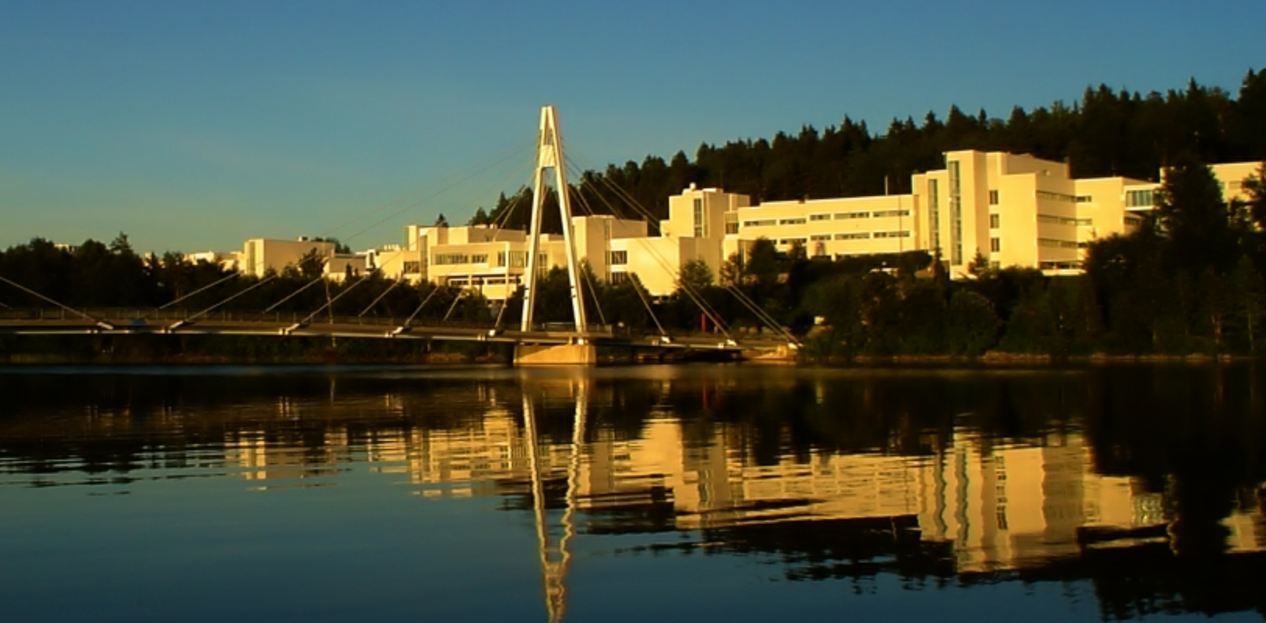
\includegraphics[scale=0.6]{assets/JYFL}
    \vfill
    \begin{textblock*}{0.3\paperwidth}(.7\paperwidth,.5\paperheight)
        \includegraphics[scale=0.07]{assets/JYFL_locator}
    \end{textblock*}
    \begin{textblock*}{0.7\paperwidth}(0.01\paperwidth,.8\paperheight)
        \color{white}{The northernmost accelerator laboratory in the world!}
    \end{textblock*}
\end{frame}

\begin{frame}{A Nuclear Physics Experiment}
    \vspace*{-4em}
    \begin{itemize}
        \item<1-| alert@1> Accelerate something (beam)
        \item<2-| alert@2> Crash it into something else (target)
        \item<3-| alert@3> See what happens (detectors)
    \end{itemize}
    \begin{textblock*}{\paperwidth}(0\paperwidth,.45\paperheight)
        \centering
        \onslide<1>{\color{primary}{K130 Cyclotron at JYFL}}
        
        \includegraphics<1>[scale=0.2]{assets/K130}
    \end{textblock*}
    \begin{textblock*}{\paperwidth}(0\paperwidth,.45\paperheight)
        \centering
               
        \includegraphics<2>[scale=.7]{assets/beamtarget}
    \end{textblock*}
    \begin{textblock*}{\paperwidth}(0\paperwidth,.45\paperheight)
        \centering
        \onslide<3>{\color{primary}{The JUROGAM Ge-detector array}}
           
        \includegraphics<3>[scale=.117]{assets/juro}
    \end{textblock*}
\end{frame}

\begin{frame}{Reactions}
    
\end{frame}

\begin{frame}{MARA}
\vspace{4em}
The Mass Analysing Recoil Apparatus (MARA) uses electric and magnetic fields to select specific recoils from fusion-evaporation reactions.

\begin{center}
    \hspace*{-1em}
    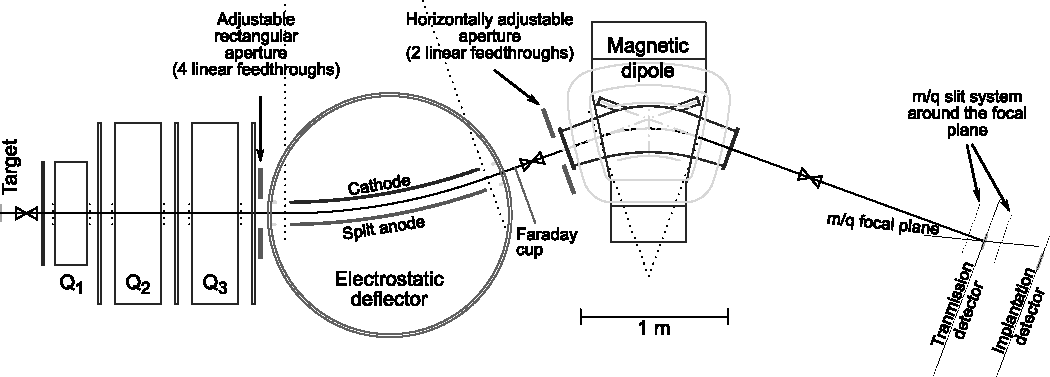
\includegraphics[scale=0.65]{assets/MARA}
\end{center}
\end{frame} 

\begin{frame}{MARA-LEB}
    \vspace{4em}
    The MARA Low Energy Branch (MARA-LEB) will be used for exotic cases to suppress background.

    It will use \alert{laser ionisation} for both measurement and purification.
    
    \begin{center}
        \hspace*{-1em}
        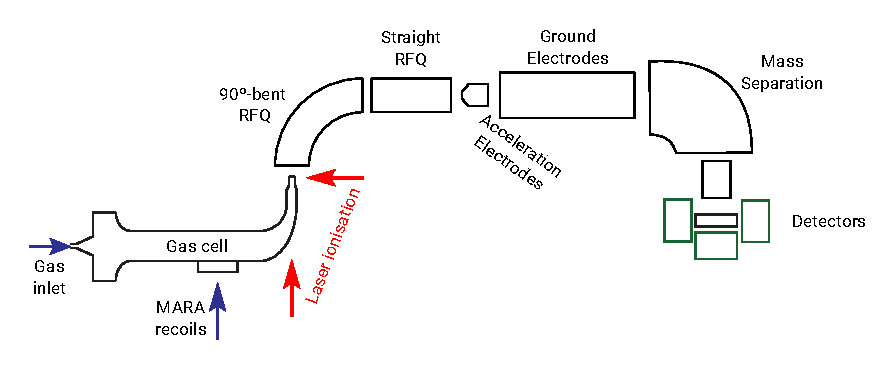
\includegraphics[scale=0.65]{assets/LEB}
    \end{center}
    \end{frame} 
\end{document}